%-----------------------------------------------------------------
%	STEERING CONTROL
%	!TEX root = ./main.tex
%-----------------------------------------------------------------
\subsection{Optimisation-based}

\begin{frame}{Optimisation-based}

\begin{onlyenv}<1>
\begin{figure}[H]
    \centering
    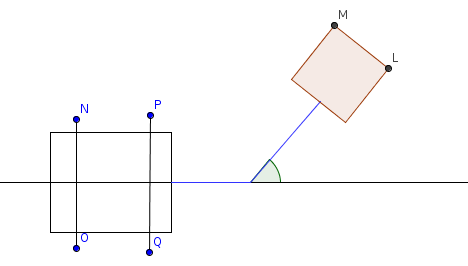
\includegraphics[width=0.55\textwidth]{images/pic_trailer.png}
    \caption{Geometric situation}
    \label{fig:trailer}
\end{figure}

\begin{figure}[H]
    \centering
    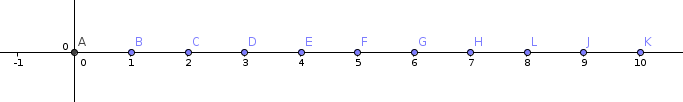
\includegraphics[width=0.55\textwidth]{images/divisions.png}
    \caption{Time divisions of the method}
    \label{fig:trailer2}
\end{figure}
% \end{frame}
\end{onlyenv}

% \begin{frame}{Frame Title}
\begin{onlyenv}<2>
We optimise, as a function of $\delta$:
\begin{align}
    \operatorname{cost}_{\alpha}(y, \phi) = y^2+\alpha \phi^2 
\end{align}

Solved using analytical expressions for the circular paths of the points in the car and using a Runge--Kutta--Fellberg 78 method to integrate the differential equation for $\phi$.
\end{onlyenv}

\begin{onlyenv}<3>
Issues with the method:
\begin{itemize}
    \item Greedy.
    \item Dependent on number of divisions and $\alpha$.
    \item One variable $\delta$ for two objectives ($y$, $\phi$).
\end{itemize}

\end{onlyenv}



\end{frame}


